% cSpell:language es,en
\documentclass[12pt,a4paper,oneside]{report}

% ==================================================================
% PREÁMBULO: Todos los paquetes y configuraciones
% ==================================================================
% ==================================================================
% ARCHIVO PRINCIPAL DE LA TESIS - main.tex
% ==================================================================
% Solo este archivo se compila. Los demás se incluyen automáticamente.

\documentclass[12pt,a4paper,twoside]{report}

% ==================================================================
% PREÁMBULO: Todos los paquetes y configuraciones
% ==================================================================
% ==================================================================
% ARCHIVO PRINCIPAL DE LA TESIS - main.tex
% ==================================================================
% Solo este archivo se compila. Los demás se incluyen automáticamente.

\documentclass[12pt,a4paper,twoside]{report}

% ==================================================================
% PREÁMBULO: Todos los paquetes y configuraciones
% ==================================================================
% ==================================================================
% ARCHIVO PRINCIPAL DE LA TESIS - main.tex
% ==================================================================
% Solo este archivo se compila. Los demás se incluyen automáticamente.

\documentclass[12pt,a4paper,twoside]{report}

% ==================================================================
% PREÁMBULO: Todos los paquetes y configuraciones
% ==================================================================
\input{preambulo.tex}

% ==================================================================
% INFORMACIÓN DEL DOCUMENTO
% ==================================================================
\title{Título de mi Tesis Doctoral}
\author{Mi Nombre Completo}
\date{\today}

% Para referencias con natbib
\bibliographystyle{apalike}

% ==================================================================
% INICIO DEL DOCUMENTO
% ==================================================================
\begin{document}

% ------------------------------------------------------------------
% PÁGINAS PRELIMINARES
% ------------------------------------------------------------------
\frontmatter  % Numeración romana para páginas preliminares

\input{portada.tex}

% Página en blanco después de portada (estilo libro)
\cleardoublepage

\input{agradecimientos.tex}
\cleardoublepage

\input{resumen.tex}
\cleardoublepage

% Tabla de contenidos
\tableofcontents
\cleardoublepage

% Lista de figuras (opcional)
\listoffigures
\cleardoublepage

% Lista de tablas (opcional)
\listoftables
\cleardoublepage

% ------------------------------------------------------------------
% CONTENIDO PRINCIPAL
% ------------------------------------------------------------------
\mainmatter  % Numeración arábiga para capítulos principales

% Incluir cada capítulo
\input{capitulos/01_introduccion.tex}
\input{capitulos/02_marco_teorico.tex}
\input{capitulos/03_metodologia.tex}
\input{capitulos/04_resultados.tex}
\input{capitulos/05_discusion.tex}
\input{capitulos/06_conclusiones.tex}

% ------------------------------------------------------------------
% BIBLIOGRAFÍA
% ------------------------------------------------------------------
\cleardoublepage
\bibliography{referencias}

% ------------------------------------------------------------------
% APÉNDICES
% ------------------------------------------------------------------
\appendix
\input{apendices/apendice_a.tex}
\input{apendices/apendice_b.tex}

\end{document}

% ==================================================================
% INFORMACIÓN DEL DOCUMENTO
% ==================================================================
\title{Título de mi Tesis Doctoral}
\author{Mi Nombre Completo}
\date{\today}

% Para referencias con natbib
\bibliographystyle{apalike}

% ==================================================================
% INICIO DEL DOCUMENTO
% ==================================================================
\begin{document}

% ------------------------------------------------------------------
% PÁGINAS PRELIMINARES
% ------------------------------------------------------------------
\frontmatter  % Numeración romana para páginas preliminares

% ==================================================================
% PORTADA
% ==================================================================

\begin{titlepage}
    \centering
    \vspace*{1cm}
    
    {\Large\textbf{\universidad}}\\[0.5cm]
    {\Large\textbf{\facultad}}\\[1.5cm]
    
    % Logo PUCP (descomentar y ajustar ruta cuando tengas la imagen)
    % 
\includegraphics[width=0.25\textwidth]{logo_pucp.png}\\[1.5cm]
    
    \vspace{1cm}
    
    {\large\textbf{DISEÑO E IMPLEMENTACIÓN DE UNA PLATAFORMA WEB Y APLICACIÓN MÓVIL CON PROCESAMIENTO DE IMÁGENES CON INTELIGENCIA ARTIFICIAL MULTIMODAL EN LA NUBE PARA LA IDENTIFICACIÓN DE PAGOS, ESTIMACIÓN DE DIMENSIONES Y OPTIMIZACIÓN LOGÍSTICA EN SERVICIOS DE DELIVERY URBANO EN LIMA}}\\[2.5cm]
    
    {\large Tesis para obtener el título profesional de}\\[0.3cm]
    {\large\textbf{Ingeniero de las Telecomunicaciones}}\\[2.5cm]
    
    {\large \textbf{Que presenta:}}\\[0.3cm]
    {\large \autor}\\[2cm]
    
    {\large \textbf{Asesor:}}\\[0.3cm]
    {\large \asesor}\\[2cm]
    
    \vfill
    
    {\large \ciudad, junio, \anio}
\end{titlepage}

% Página en blanco después de portada (estilo libro)
\cleardoublepage

\chapter*{AGRADECIMIENTOS}
\addcontentsline{toc}{chapter}{AGRADECIMIENTOS}
[Por completar]
\cleardoublepage

\chapter*{RESUMEN}
\addcontentsline{toc}{chapter}{RESUMEN}
[Por completar]
\cleardoublepage

% Tabla de contenidos
\tableofcontents
\cleardoublepage

% Lista de figuras (opcional)
\listoffigures
\cleardoublepage

% Lista de tablas (opcional)
\listoftables
\cleardoublepage

% ------------------------------------------------------------------
% CONTENIDO PRINCIPAL
% ------------------------------------------------------------------
\mainmatter  % Numeración arábiga para capítulos principales

% Incluir cada capítulo
% cSpell:language es,en
% ==================================================================
% CAPÍTULO 1: INTRODUCCIÓN
% ==================================================================
\chapter{Introducción}

% ------------------------------------------------------------------
% SECCIÓN: Planteamiento del problema
% ------------------------------------------------------------------
\section{Planteamiento del problema}

En los últimos años, el desarrollo de nuevas tecnologías ha transformado significativamente el panorama de la investigación científica \citep{autor2023}. Este fenómeno presenta tanto oportunidades como desafíos que requieren un análisis profundo.

El problema central de esta investigación se puede formular mediante la siguiente pregunta: ¿Cómo puede optimizarse el proceso de análisis de datos utilizando técnicas de machine learning para mejorar la precisión de los resultados?

% ------------------------------------------------------------------
% SECCIÓN: Justificación
% ------------------------------------------------------------------
\section{Justificación}

La relevancia de este estudio radica en varios aspectos fundamentales:

\begin{itemize}
    \item \textbf{Relevancia teórica}: Contribuye al conocimiento existente sobre métodos de análisis de datos.
    \item \textbf{Relevancia práctica}: Proporciona herramientas aplicables en contextos reales.
    \item \textbf{Relevancia metodológica}: Introduce nuevas técnicas de investigación.
\end{itemize}

Según \citet{otroautor2022}, los avances en este campo pueden tener un impacto significativo en múltiples disciplinas.

% ------------------------------------------------------------------
% SECCIÓN: Objetivos
% ------------------------------------------------------------------
\section{Objetivos}

\subsection{Objetivo general}

Desarrollar e implementar un framework de análisis de datos que integre técnicas de machine learning para mejorar la precisión y eficiencia en el procesamiento de información científica.

\subsection{Objetivos específicos}

\begin{enumerate}
    \item Realizar un análisis exhaustivo del estado del arte en técnicas de machine learning aplicadas al análisis de datos científicos.
    \item Diseñar una arquitectura de software que permita la integración de múltiples algoritmos de aprendizaje automático.
    \item Implementar el framework propuesto y validarlo mediante casos de estudio específicos.
    \item Evaluar el rendimiento del sistema desarrollado comparándolo con métodos tradicionales.
\end{enumerate}

% ------------------------------------------------------------------
% SECCIÓN: Hipótesis
% ------------------------------------------------------------------
\section{Hipótesis}

\textbf{Hipótesis principal}: La implementación de un framework integrado de machine learning mejorará significativamente la precisión del análisis de datos científicos en comparación con métodos tradicionales.

\textbf{Hipótesis específicas}:
\begin{itemize}
    \item H1: El framework propuesto reducirá el tiempo de procesamiento en al menos un 30\%.
    \item H2: La precisión de los resultados se incrementará en un mínimo de 15\%.
    \item H3: La usabilidad del sistema será superior a las herramientas existentes.
\end{itemize}

% ------------------------------------------------------------------
% SECCIÓN: Limitaciones del estudio
% ------------------------------------------------------------------
\section{Limitaciones del estudio}

Este estudio presenta las siguientes limitaciones:

\begin{description}
    \item[Temporal] La investigación se llevó a cabo durante un período de 2 años, lo que puede limitar la generalización de algunos resultados.
    \item[Poblacional] Los casos de estudio se centraron en datos provenientes de un dominio específico.
    \item[Tecnológica] Se utilizaron únicamente herramientas de código abierto disponibles al momento de la investigación.
\end{description}

\input{capitulos/02_marco_teorico.tex}
% cSpell:language es,en
% ==================================================================
% CAPÍTULO 3: ESTADO DEL ARTE
% ==================================================================
\chapter{Estado del arte o de la cuestión, alternativas de solución al problema o desafío a resolver}
\input{capitulos/04_resultados.tex}
\input{capitulos/05_discusion.tex}
\input{capitulos/06_conclusiones.tex}

% ------------------------------------------------------------------
% BIBLIOGRAFÍA
% ------------------------------------------------------------------
\cleardoublepage
\bibliography{referencias}

% ------------------------------------------------------------------
% APÉNDICES
% ------------------------------------------------------------------
\appendix
\input{apendices/apendice_a.tex}
\input{apendices/apendice_b.tex}

\end{document}

% ==================================================================
% INFORMACIÓN DEL DOCUMENTO
% ==================================================================
\title{Título de mi Tesis Doctoral}
\author{Mi Nombre Completo}
\date{\today}

% Para referencias con natbib
\bibliographystyle{apalike}

% ==================================================================
% INICIO DEL DOCUMENTO
% ==================================================================
\begin{document}

% ------------------------------------------------------------------
% PÁGINAS PRELIMINARES
% ------------------------------------------------------------------
\frontmatter  % Numeración romana para páginas preliminares

% ==================================================================
% PORTADA
% ==================================================================

\begin{titlepage}
    \centering
    \vspace*{1cm}
    
    {\Large\textbf{\universidad}}\\[0.5cm]
    {\Large\textbf{\facultad}}\\[1.5cm]
    
    % Logo PUCP (descomentar y ajustar ruta cuando tengas la imagen)
    % 
\includegraphics[width=0.25\textwidth]{logo_pucp.png}\\[1.5cm]
    
    \vspace{1cm}
    
    {\large\textbf{DISEÑO E IMPLEMENTACIÓN DE UNA PLATAFORMA WEB Y APLICACIÓN MÓVIL CON PROCESAMIENTO DE IMÁGENES CON INTELIGENCIA ARTIFICIAL MULTIMODAL EN LA NUBE PARA LA IDENTIFICACIÓN DE PAGOS, ESTIMACIÓN DE DIMENSIONES Y OPTIMIZACIÓN LOGÍSTICA EN SERVICIOS DE DELIVERY URBANO EN LIMA}}\\[2.5cm]
    
    {\large Tesis para obtener el título profesional de}\\[0.3cm]
    {\large\textbf{Ingeniero de las Telecomunicaciones}}\\[2.5cm]
    
    {\large \textbf{Que presenta:}}\\[0.3cm]
    {\large \autor}\\[2cm]
    
    {\large \textbf{Asesor:}}\\[0.3cm]
    {\large \asesor}\\[2cm]
    
    \vfill
    
    {\large \ciudad, junio, \anio}
\end{titlepage}

% Página en blanco después de portada (estilo libro)
\cleardoublepage

\chapter*{AGRADECIMIENTOS}
\addcontentsline{toc}{chapter}{AGRADECIMIENTOS}
[Por completar]
\cleardoublepage

\chapter*{RESUMEN}
\addcontentsline{toc}{chapter}{RESUMEN}
[Por completar]
\cleardoublepage

% Tabla de contenidos
\tableofcontents
\cleardoublepage

% Lista de figuras (opcional)
\listoffigures
\cleardoublepage

% Lista de tablas (opcional)
\listoftables
\cleardoublepage

% ------------------------------------------------------------------
% CONTENIDO PRINCIPAL
% ------------------------------------------------------------------
\mainmatter  % Numeración arábiga para capítulos principales

% Incluir cada capítulo
% cSpell:language es,en
% ==================================================================
% CAPÍTULO 1: INTRODUCCIÓN
% ==================================================================
\chapter{Introducción}

% ------------------------------------------------------------------
% SECCIÓN: Planteamiento del problema
% ------------------------------------------------------------------
\section{Planteamiento del problema}

En los últimos años, el desarrollo de nuevas tecnologías ha transformado significativamente el panorama de la investigación científica \citep{autor2023}. Este fenómeno presenta tanto oportunidades como desafíos que requieren un análisis profundo.

El problema central de esta investigación se puede formular mediante la siguiente pregunta: ¿Cómo puede optimizarse el proceso de análisis de datos utilizando técnicas de machine learning para mejorar la precisión de los resultados?

% ------------------------------------------------------------------
% SECCIÓN: Justificación
% ------------------------------------------------------------------
\section{Justificación}

La relevancia de este estudio radica en varios aspectos fundamentales:

\begin{itemize}
    \item \textbf{Relevancia teórica}: Contribuye al conocimiento existente sobre métodos de análisis de datos.
    \item \textbf{Relevancia práctica}: Proporciona herramientas aplicables en contextos reales.
    \item \textbf{Relevancia metodológica}: Introduce nuevas técnicas de investigación.
\end{itemize}

Según \citet{otroautor2022}, los avances en este campo pueden tener un impacto significativo en múltiples disciplinas.

% ------------------------------------------------------------------
% SECCIÓN: Objetivos
% ------------------------------------------------------------------
\section{Objetivos}

\subsection{Objetivo general}

Desarrollar e implementar un framework de análisis de datos que integre técnicas de machine learning para mejorar la precisión y eficiencia en el procesamiento de información científica.

\subsection{Objetivos específicos}

\begin{enumerate}
    \item Realizar un análisis exhaustivo del estado del arte en técnicas de machine learning aplicadas al análisis de datos científicos.
    \item Diseñar una arquitectura de software que permita la integración de múltiples algoritmos de aprendizaje automático.
    \item Implementar el framework propuesto y validarlo mediante casos de estudio específicos.
    \item Evaluar el rendimiento del sistema desarrollado comparándolo con métodos tradicionales.
\end{enumerate}

% ------------------------------------------------------------------
% SECCIÓN: Hipótesis
% ------------------------------------------------------------------
\section{Hipótesis}

\textbf{Hipótesis principal}: La implementación de un framework integrado de machine learning mejorará significativamente la precisión del análisis de datos científicos en comparación con métodos tradicionales.

\textbf{Hipótesis específicas}:
\begin{itemize}
    \item H1: El framework propuesto reducirá el tiempo de procesamiento en al menos un 30\%.
    \item H2: La precisión de los resultados se incrementará en un mínimo de 15\%.
    \item H3: La usabilidad del sistema será superior a las herramientas existentes.
\end{itemize}

% ------------------------------------------------------------------
% SECCIÓN: Limitaciones del estudio
% ------------------------------------------------------------------
\section{Limitaciones del estudio}

Este estudio presenta las siguientes limitaciones:

\begin{description}
    \item[Temporal] La investigación se llevó a cabo durante un período de 2 años, lo que puede limitar la generalización de algunos resultados.
    \item[Poblacional] Los casos de estudio se centraron en datos provenientes de un dominio específico.
    \item[Tecnológica] Se utilizaron únicamente herramientas de código abierto disponibles al momento de la investigación.
\end{description}

\input{capitulos/02_marco_teorico.tex}
% cSpell:language es,en
% ==================================================================
% CAPÍTULO 3: ESTADO DEL ARTE
% ==================================================================
\chapter{Estado del arte o de la cuestión, alternativas de solución al problema o desafío a resolver}
\input{capitulos/04_resultados.tex}
\input{capitulos/05_discusion.tex}
\input{capitulos/06_conclusiones.tex}

% ------------------------------------------------------------------
% BIBLIOGRAFÍA
% ------------------------------------------------------------------
\cleardoublepage
\bibliography{referencias}

% ------------------------------------------------------------------
% APÉNDICES
% ------------------------------------------------------------------
\appendix
\input{apendices/apendice_a.tex}
\input{apendices/apendice_b.tex}

\end{document}

% ==================================================================
% INFORMACIÓN DEL DOCUMENTO
% ==================================================================
\title{Diseño e Implementación de una Plataforma Web y Aplicación Móvil con Procesamiento de Imágenes con Inteligencia Artificial Multimodal en la Nube para la Identificación de Pagos, Estimación de Dimensiones y Optimización Logística en Servicios de Delivery Urbano en Lima}
\author{Juan Alfonso Chapoñan Espinoza}
\date{Lima, junio, 2025}

% ==================================================================
% INICIO DEL DOCUMENTO
% ==================================================================
\begin{document}

% ------------------------------------------------------------------
% PÁGINAS PRELIMINARES
% ------------------------------------------------------------------
\frontmatter  % Numeración romana para páginas preliminares

% ==================================================================
% PORTADA
% ==================================================================

\begin{titlepage}
    \centering
    \vspace*{1cm}
    
    {\Large\textbf{\universidad}}\\[0.5cm]
    {\Large\textbf{\facultad}}\\[1.5cm]
    
    % Logo PUCP (descomentar y ajustar ruta cuando tengas la imagen)
    % 
\includegraphics[width=0.25\textwidth]{logo_pucp.png}\\[1.5cm]
    
    \vspace{1cm}
    
    {\large\textbf{DISEÑO E IMPLEMENTACIÓN DE UNA PLATAFORMA WEB Y APLICACIÓN MÓVIL CON PROCESAMIENTO DE IMÁGENES CON INTELIGENCIA ARTIFICIAL MULTIMODAL EN LA NUBE PARA LA IDENTIFICACIÓN DE PAGOS, ESTIMACIÓN DE DIMENSIONES Y OPTIMIZACIÓN LOGÍSTICA EN SERVICIOS DE DELIVERY URBANO EN LIMA}}\\[2.5cm]
    
    {\large Tesis para obtener el título profesional de}\\[0.3cm]
    {\large\textbf{Ingeniero de las Telecomunicaciones}}\\[2.5cm]
    
    {\large \textbf{Que presenta:}}\\[0.3cm]
    {\large \autor}\\[2cm]
    
    {\large \textbf{Asesor:}}\\[0.3cm]
    {\large \asesor}\\[2cm]
    
    \vfill
    
    {\large \ciudad, junio, \anio}
\end{titlepage}
\cleardoublepage

% Informe de Similitud
\chapter*{INFORME DE SIMILITUD}
%\addcontentsline{toc}{chapter}{Informe de Similitud}

\vspace{1cm}

Yo, \textbf{OSCAR ANTONIO DÍAZ BARRIGA}, docente de la Facultad de \textbf{CIENCIAS E INGENIERÍA} de la Pontificia Universidad Católica del Perú, asesor de la tesis titulada \textbf{PLATAFORMA WEB Y MÓVIL CON PROCESAMIENTO DE IMÁGENES EN LA NUBE E INTELIGENCIA ARTIFICIAL PARA LA IDENTIFICACIÓN DE PAGOS, ESTIMACIÓN DE DIMENSIONES Y OPTIMIZACIÓN LOGÍSTICA EN SERVICIOS DE DELIVERY URBANO EN LIMA}, del autor \textbf{JUAN ALFONSO CHAPOÑAN ESPINOZA}, dejo constancia de lo siguiente:

\begin{itemize}
    \item El mencionado documento tiene un índice de puntuación de similitud de \textbf{[\#\#]\%}. Así lo consigna el reporte de similitud emitido por el software Turnitin el \textbf{[DD/MM/AAAA]}.
    
    \item He revisado con detalle dicho reporte y la Tesis, y no se advierte indicios de plagio.
    
    \item Las citas a otros autores y sus respectivas referencias cumplen con las pautas académicas.
\end{itemize}

\vspace{1.5cm}

\textbf{Lugar y fecha:} San Miguel, [DD] de [MES] de [AAAA].

\vspace{2cm}

\begin{table}[H]
\centering
\begin{tabular}{|p{7cm}|p{7cm}|}
\hline
Apellidos y nombres del asesor: & \\
\textbf{DÍAZ BARRIGA, OSCAR ANTONIO} & \\
\hline
DNI: \textbf{71477000} & Firma \\
\hline
ORCID: 0000-0002-9930-5984 & \\
\hline
\end{tabular}
\end{table}

\cleardoublepage

% Dedicatoria
\chapter*{DEDICATORIA}
\addcontentsline{toc}{chapter}{DEDICATORIA}
A mis padres.

\cleardoublepage

% Agradecimientos
\chapter*{AGRADECIMIENTOS}
\addcontentsline{toc}{chapter}{AGRADECIMIENTOS}
[Por completar]
\cleardoublepage

% Resumen y Abstract
\chapter*{RESUMEN}
\addcontentsline{toc}{chapter}{RESUMEN}
[Por completar]
\cleardoublepage

% Tabla de contenidos
\tableofcontents
\cleardoublepage

% Lista de tablas
\listoftables
\cleardoublepage

% Lista de figuras
\listoffigures
\cleardoublepage

% Glosario
\chapter*{GLORASIO}
\addcontentsline{toc}{chapter}{GLOSARIO}
[Por completar]
\cleardoublepage

% ------------------------------------------------------------------
% CONTENIDO PRINCIPAL
% ------------------------------------------------------------------
\mainmatter  % Numeración arábiga para capítulos principales

% Introducción (sin número de capítulo)
\chapter*{INTRODUCCIÓN}
\addcontentsline{toc}{chapter}{INTRODUCCIÓN}
[Por completar]


% Capítulos numerados
% cSpell:language es,en
% ==================================================================
% CAPÍTULO 1: PRESENTACIÓN DEL PROBLEMA DE INGENIERÍA
% ==================================================================

\chapter{Presentación del problema de ingeniería}

La transformación digital en el sector logístico demanda soluciones innovadoras que aprovechen tecnologías emergentes para resolver desafíos operacionales críticos. Esta investigación aborda la problemática de la inexactitud en la determinación de dimensiones de paquetes en la industria de \textit{delivery}, factor que genera ineficiencias significativas en la planificación de rutas y utilización de capacidad vehicular. Mediante la convergencia de aplicaciones IoT, procesamiento de imágenes con inteligencia artificial y arquitecturas distribuidas en la nube, se propone una solución integral que mejora la precisión operacional y democratiza el acceso a tecnologías sofisticadas para empresas de diferentes escalas.

% ------------------------------------------------------------------
\section{Identificación temática y motivación personal}
% ------------------------------------------------------------------

\subsection{Área de especialización en telecomunicaciones}

\subsubsection{Aplicaciones IoT (\textit{Internet of Things})}

Las aplicaciones IoT constituyen un ecosistema tecnológico integral que integra inteligencia artificial, redes de comunicación y automatización para crear una infraestructura de conectividad ubicua entre objetos físicos y sistemas digitales \cite{Liu2013}. Se define como la implementación de una arquitectura de cinco capas interconectadas:

\begin{table}[H]
\centering
\caption{Arquitectura IoT \cite{Zhou2022}.}
\label{tab:arquitectura_iot}
\begin{tabular}{@{}ll@{}}
\toprule
\textbf{Capa} & \textbf{Descripción} \\
\midrule
Percepción & Sensores y dispositivos de captura \\
Red & Protocolos de comunicación y transmisión \\
Middleware & Procesamiento y almacenamiento de datos \\
Aplicación & Servicios e interfaces de usuario \\
Negocio & Análisis y toma de decisiones \\
\bottomrule
\end{tabular}
\end{table}

\subsubsection{Servicios de Telecomunicaciones para Logística}

Los servicios de telecomunicaciones para logística se definen como el conjunto de tecnologías y protocolos de comunicación que operan principalmente en la capa de red del ecosistema IoT, actuando como puente crítico entre la percepción de datos y su procesamiento funcional. Estos servicios garantizan la transmisión eficiente y segura de información tanto estática como móvil durante todas las fases del proceso logístico \cite{Zhou2022}.

\subsubsection{Convergencia Tecnológica}

La tesis desarrollada en esta investigación representa la convergencia de múltiples disciplinas dentro de la ingeniería de telecomunicaciones:

\begin{itemize}
    \item \textbf{Arquitecturas Distribuidas en la Nube}: Para el procesamiento remoto y almacenamiento escalable
    \item \textbf{Inteligencia Artificial}: Específicamente visión por computadora para el procesamiento automatizado de imágenes
\end{itemize}

Esta integración tecnológica permite abordar desafíos reales del sector logístico mediante soluciones que aprovechan las capacidades de procesamiento remoto, almacenamiento distribuido y comunicaciones continuas, características fundamentales de los sistemas modernos de telecomunicaciones en el contexto de la transformación digital.

% ------------------------------------------------------------------
\subsection{Relación con los estudios realizados}
% ------------------------------------------------------------------

La presente investigación se fundamenta en una progresión curricular especializada que abarca desde los fundamentos del desarrollo web hasta la implementación de soluciones IoT avanzadas, estableciendo una relación directa y sistemática con tres cursos clave que proporcionan las competencias técnicas necesarias.

\subsubsection{TEL131 Ingeniería Web para Telecomunicaciones}

Este curso proporciona la base tecnológica para desarrollar la capa de aplicación e interfaces de gestión en soluciones de logística inteligente. Se abordan fundamentos de programación, desarrollo web con conexión a bases de datos, y modelado relacional con SQL, aplicables en \textit{dashboards} para monitoreo en tiempo real, interfaces de control y manejo de datos IoT.

\subsubsection{TEL137 Gestión de Servicios de TICs}

Este curso se enfoca en la gestión de servicios dentro del ecosistema IoT, brindando competencias para desarrollar infraestructuras seguras, escalables y robustas. A través de \textit{frameworks} modernos y servicios web, se construyen sistemas capaces de optimizar rutas y asignar recursos inteligentemente.

\subsubsection{1TEL05 Servicios y Aplicaciones para IoT}

Este curso se centra en la construcción de la capa de aplicación IoT y su integración con la nube, facilitando el desarrollo de soluciones logísticas orientadas al usuario final. Se abordan competencias en aplicaciones móviles conectadas a servicios SaaS, útiles para rastreo de productos y alertas inteligentes.

% ------------------------------------------------------------------
\subsection{Motivación personal y experiencia profesional}
% ------------------------------------------------------------------

La motivación personal para abordar esta problemática combina una vocación por la automatización de procesos con un interés social en mejorar la eficiencia empresarial. La experiencia profesional durante la carrera, desde almacenero hasta asistente logístico, brindó una comprensión directa de los desafíos operacionales, destacando la importancia del cumplimiento de tiempos en cada etapa del proceso logístico.

% ------------------------------------------------------------------
\section{Descripción y características del problema}
% ------------------------------------------------------------------

\subsection{Contexto del problema en la industria de \textit{delivery}}

La industria de servicios de \textit{delivery} y logística de última milla ha experimentado un crecimiento exponencial en los últimos años, impulsada por el auge del comercio electrónico y los cambios en los hábitos de consumo de la población \cite{RedacciponTLW2025}. 

\begin{table}[H]
\centering
\caption{Proyecciones del Mercado de delivery en Perú.}
\label{tab:proyecciones_delivery}
\begin{tabular}{@{}lcc@{}}
\toprule
\textbf{Año} & \textbf{Crecimiento (\%)} & \textbf{Ingresos (millones USD)} \\
\midrule
2024 & --- & 2,500 \\
2029 & 11.03 & 2,951 \\
\bottomrule
\end{tabular}
\end{table}

Uno de los principales desafíos que enfrentan las empresas de \textit{delivery} es obtener información precisa sobre las dimensiones y características de los paquetes que deben recoger y entregar.

\subsection{Desafío técnico desde la perspectiva de telecomunicaciones}

Desde la perspectiva de la ingeniería de telecomunicaciones, el problema central radica en la necesidad de desarrollar un sistema distribuido que permita el procesamiento automatizado de imágenes capturadas por dispositivos móviles para la determinación precisa de dimensiones de paquetes.

\subsection{Características específicas del problema}

El problema presenta características específicas que lo hacen particularmente complejo desde el punto de vista técnico y operacional:

\begin{itemize}
    \item Gran variabilidad en dimensiones, formas y características físicas de los paquetes
    \item Limitación de capacidad de los motorizados
    \item Necesidad de confiabilidad en los procesos de verificación
    \item Requisito de escalabilidad del sistema
\end{itemize}

% ------------------------------------------------------------------
\section{Importancia del problema y su solución}
% ------------------------------------------------------------------

\subsection{Perspectiva técnica}

Resolver este problema es clave por el uso de tecnologías emergentes que transforman telecomunicaciones y computación distribuida. El procesamiento en la nube ha madurado para realizar análisis complejos de imágenes sin necesidad de ejecución local en dispositivos \cite{Xu2012,Wang2012}.

\subsection{Perspectiva económica y financiera}

La automatización en medición de paquetes mejora rentabilidad y competitividad logística, generando ahorros significativos y optimizando recursos de transporte \cite{Krysiska2024}.

\begin{figure}[H]
    \centering
    % \includegraphics[width=0.8\textwidth]{gastos_tecnologia.png}
    \caption{Gasto en tecnologías de la información - América Latina.}
    \label{fig:gastos_tecnologia}
\end{figure}

\subsection{Perspectiva social y cultural}

Socialmente, la solución mejora la calidad de vida de trabajadores logísticos y usuarios finales. La automatización de tareas repetitivas permite enfocar recursos humanos en actividades de mayor valor, mejorando satisfacción laboral y desarrollo profesional.

\subsection{Perspectiva ambiental y de sostenibilidad}

Abordar este problema es clave para reducir emisiones de gases de efecto invernadero y usar recursos energéticos eficientemente. La optimización de rutas, basada en medidas precisas de paquetes, permite planificar trayectos más cortos, disminuyendo consumo de combustible y emisiones de CO₂.

\subsection{Perspectiva legal y reglamentaria}

En Perú, la medición automatizada de paquetes con IoT debe cumplir la Ley N.º 29733, que exige consentimiento previo, finalidad clara, calidad y seguridad en el tratamiento de datos \cite{EditoraPer2973}.

\subsection{Perspectiva ética}

La automatización plantea dilemas éticos sobre responsabilidad social, equidad digital, sostenibilidad ambiental, privacidad de datos y rendición de cuentas. Esta visión ética integral asegura que la tecnología respete valores humanos y apoye un desarrollo sostenible.

% ------------------------------------------------------------------
\section{Impactos previstos y beneficiarios}
% ------------------------------------------------------------------

\subsection{Impactos operacionales}

La implementación tendrá impactos operacionales significativos, mejorando la eficiencia mediante tecnologías IoT, IA y visión artificial \cite{RedaccinTLW2024,Alharbi2023}.

\subsubsection{Reducción de tiempos de procesamiento}

La medición automatizada elimina procesos manuales, reduciendo el tiempo requerido para registrar, verificar y procesar solicitudes \cite{Xu2012}.

\subsubsection{Optimización de rutas de entrega}

Con datos precisos sobre dimensiones, los sistemas pueden planificar rutas más eficientes considerando capacidad de carga, tiempo y distancia.

\subsection{Impactos tecnológicos}

La implementación tendrá un impacto tecnológico significativo en telecomunicaciones e IoT, estableciendo nuevos paradigmas en procesamiento de imágenes para logística.

\subsection{Impactos económicos}

Los impactos económicos se reflejan desde la productividad individual hasta la competitividad sectorial, aprovechando procesamiento de imágenes con IA en la nube para optimizar entregas urbanas.

\subsection{Beneficiarios directos}

\subsubsection{Empresas de \textit{delivery} y logística}

Son los principales beneficiarios, mejorando eficiencia y rentabilidad gracias al procesamiento de imágenes con IA en la nube.

\subsubsection{Motorizados y personal operativo}

Mejoran productividad y condiciones laborales mediante rutas optimizadas que permiten más entregas en menos tiempo.

\subsubsection{Clientes emisores de paquetes}

Experimentan mayor fiabilidad y transparencia con rutas inteligentes que optimizan entregas y recojo.

\subsubsection{Destinatarios de entregas}

Reciben un servicio más rápido y predecible, cumpliendo estándares de \textit{quick commerce} en menos de 90 minutos.

\subsection{Beneficiarios indirectos}

\subsubsection{Sector de Telecomunicaciones}

Este sector verá un aumento en la demanda de servicios especializados y mejoras en infraestructura.

\subsubsection{Industria de Desarrollo de Software}

Se generarán nuevas oportunidades y mayor demanda de talento especializado en aplicaciones móviles, NoSQL y microservicios.

\subsubsection{Medio Ambiente y Sociedad}

La optimización de rutas reducirá emisiones de CO₂ y consumo de combustible, contribuyendo a un entorno urbano más saludable.

\subsubsection{Ecosistema de Innovación Tecnológica}

La solución fortalecerá la innovación al demostrar cómo tecnologías emergentes resuelven problemas reales.
% cSpell:language es,en
% ==================================================================
% CAPÍTULO 2: ESTADO DEL ARTE
% ==================================================================

\chapter{Estado del arte o de la cuestión, alternativas de solución al problema o desafío a resolver}

% ------------------------------------------------------------------
\section{Antecedentes de solución semejantes o similares al desafío de ingeniería}
% ------------------------------------------------------------------

\subsection{Sistemas de análisis visual con inteligencia artificial multimodal}

\subsubsection{Caso 1: GPT-4 Vision para análisis de objetos (OpenAI, Estados Unidos, 2023)}

GPT-4 Vision, lanzado en septiembre de 2023, representa el primer modelo de lenguaje de gran escala con capacidades multimodal nativas de OpenAI. El sistema demuestra capacidades avanzadas de interpretación visual con un 95\% de precisión en reconocimiento de objetos comunes y 78.5\% de efectividad en análisis de gráficos complejos según evaluaciones técnicas independientes \cite{ArticleRef255136}.

En términos de estimación dimensional, GPT-4V utiliza razonamiento contextual para comparar tamaños relativos entre objetos, empleando elementos conocidos como referencias de escala. Las evaluaciones técnicas reportan una precisión de $\pm$15--25\% de error en estimaciones dimensionales cuando se proporcionan referencias visuales adecuadas, mejorando a $\pm$10--20\% bajo condiciones de iluminación controlada \cite{Yu2024}.

\begin{figure}[H]
    \centering
    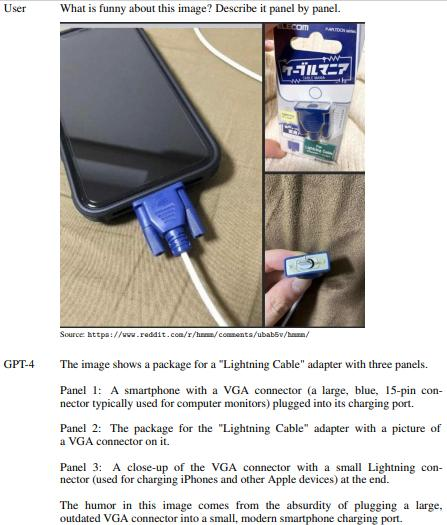
\includegraphics[width=0.9\textwidth]{gpt4_vision_example.png}
    \caption{Consulta a GPT-4 para análisis de múltiples imágenes. Fuente \cite{ArticleRef255134}}
    \label{fig:gpt4_vision}
\end{figure}

La arquitectura se basa en un \textit{transformer} multimodal que integra un codificador visual especializado con el modelo de lenguaje GPT-4, estimado en 1.76 trillones de parámetros. El sistema procesa imágenes de hasta 2048$\times$2048 píxeles en formatos JPEG, PNG, GIF y WebP, utilizando técnicas de atención cruzada para correlacionar información visual con conocimiento lingüístico \cite{ArticleRef255134}.

El modelo emplea un enfoque de \textit{vision-language understanding} que permite no solo identificar objetos, sino también razonar sobre sus propiedades físicas, relaciones espaciales y características dimensionales mediante una interpretación contextual similar al razonamiento humano \cite{ArticleRef255136}.

Las evaluaciones técnicas del sistema revelan un rendimiento variable según el contexto de aplicación:

\begin{itemize}
    \item MMMU \textit{Benchmark}: 56.8\% en tareas multimodal complejas
    \item \textit{MathVista}: 49.9\% en razonamiento visual-matemático
    \item AI2D: 78.2\% en interpretación de diagramas técnicos
    \item ChartQA: 78.5\% en análisis de gráficos y visualizaciones
\end{itemize}

Para tareas específicas de estimación dimensional, el sistema muestra mejor rendimiento en cajas rectangulares estándar, objetos con formas geométricas simples y productos comerciales conocidos, alcanzando precisiones útiles para la categorización logística y la clasificación de tarifas de envío \cite{Yu2024}.

Las evaluaciones técnicas identifican limitaciones significativas en aplicaciones que requieren precisión cuantitativa absoluta:

\begin{itemize}
    \item \textbf{Sin calibración externa:} incremento del error a $\pm$30--50\% en ausencia de referencias de escala conocidas.
    \item \textbf{Sensibilidad ambiental:} degradación de precisión con variaciones en iluminación, ángulos de captura y condiciones visuales.
    \item \textbf{Limitaciones de escala:} rendimiento reducido en objetos menores a 5\,cm o con formas irregulares complejas.
    \item \textbf{Objetos problemáticos:} dificultades con elementos transparentes, reflectivos o sin texturas distintivas.
\end{itemize}

El \textit{GPT-4V System Card} oficial de OpenAI reconoce explícitamente que “el modelo no está optimizado para mediciones precisas y puede proporcionar estimaciones aproximadas que requieren validación adicional para aplicaciones críticas” \cite{ArticleRef255136}.


\subsubsection{Caso 2: Claude 3 Vision}

Claude 3, lanzado en marzo de 2024 en sus variantes Haiku, Sonnet y Opus, establece un nuevo estándar en interpretación multimodal con un enfoque específico en razonamiento avanzado sobre contenido visual complejo. El sistema demuestra capacidades superiores a GPT-4V en interpretación de gráficos y documentos técnicos, alcanzando un 86.8\% en el benchmark MMLU y un 60.1\% en problemas matemáticos complejos con componentes visuales \cite{Anthropic2024}.

La arquitectura del modelo incorpora una ventana de contexto extendida de 200{,}000 tokens que incluye contenido visual, permitiendo el análisis simultáneo de múltiples imágenes y documentos dentro de una sola conversación. Esta capacidad es particularmente relevante para el análisis de inventarios complejos, donde se requiere correlacionar información entre múltiples fuentes visuales \cite{WebRef13251}.

\begin{figure}[H]
    \centering
    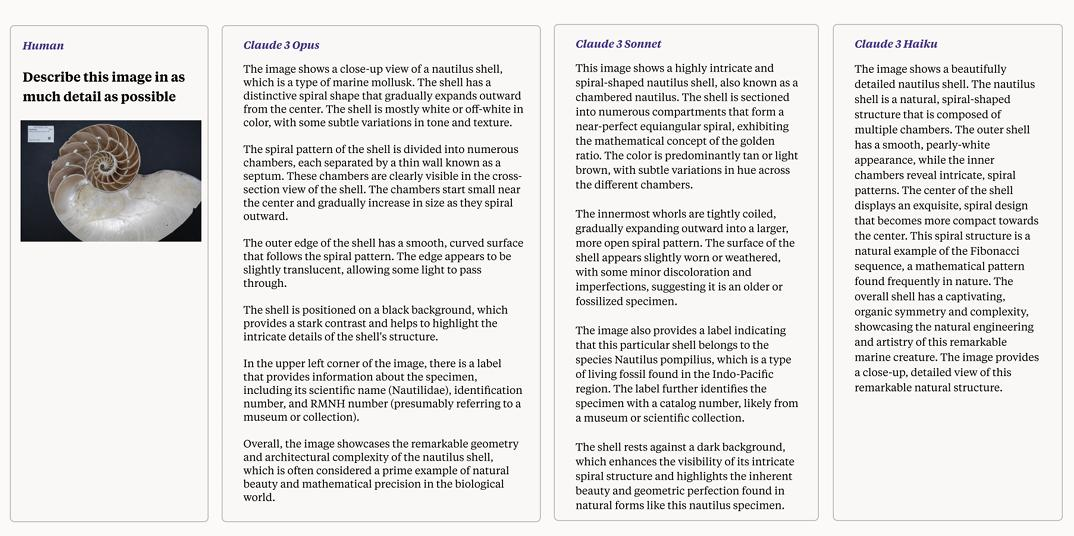
\includegraphics[width=0.85\textwidth]{claude3_vision_detection.png}
    \caption{Identificación de objetos visualmente usando modelos de Claude 3. Fuente: \cite{Anthropic2024}}
    \label{fig:claude3_detection}
\end{figure}

Claude 3 destaca en el reconocimiento óptico de caracteres (\textit{OCR}) en imágenes complejas, el procesamiento de documentos técnicos con \textit{layouts} sofisticados y la comprensión contextual de diagramas industriales, superando consistentemente a modelos anteriores en \textit{benchmarks} de comprensión documental \cite{Anthropic2024}.

El modelo exhibe capacidades avanzadas de razonamiento espacial que superan a sus predecesores en tareas que requieren comprensión de relaciones geométricas y propiedades físicas de objetos. Las evaluaciones técnicas independientes reportan un rendimiento superior en tareas de razonamiento espacial, con particular fortaleza en la interpretación de \textit{layouts} complejos y relaciones proporcionales entre elementos.

\begin{figure}[H]
    \centering
    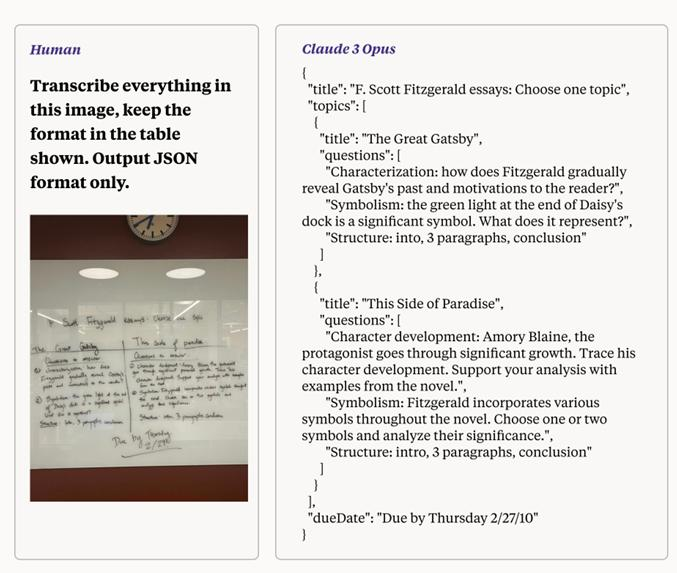
\includegraphics[width=0.85\textwidth]{claude3_json_output.png}
    \caption{Solicitud de reconocimiento de una imagen y reorganización en formato JSON.Fuente: \cite{Anthropic2024}}
    \label{fig:claude3_json}
\end{figure}

Para estimación dimensional, Claude 3 utiliza razonamiento contextual sofisticado que combina el reconocimiento de objetos conocidos con el análisis proporcional de elementos en la imagen. El sistema puede interpretar planos técnicos con dimensiones especificadas y extrapolar esta información para estimar las dimensiones de objetos fotografiados, logrando precisiones de $\pm$20--30\% en estimaciones sin referencias calibradas externas \cite{WebRef13251}.

La capacidad de procesamiento de documentos técnicos permite al modelo analizar especificaciones de productos, diagramas de embalaje y planos industriales, proporcionando estimaciones dimensionales basadas en la información contextual disponible en los documentos \cite{Anthropic2024}.

Claude 3 ofrece integración empresarial a través de la \textit{Anthropic API v1}, que proporciona \textit{endpoints RESTful} con autenticación basada en \textit{API keys} y límites de 4{,}000 tokens por minuto para todas las variantes del modelo. La \textit{API} soporta imágenes de hasta 20\,MB en formatos JPEG, PNG, GIF, WebP y PDF, facilitando la integración con sistemas existentes de gestión documental.

La arquitectura de la \textit{API} permite respuestas en múltiples formatos estructurados, incluyendo \textit{JSON}, texto estructurado y \textit{Markdown}, lo que facilita la integración con sistemas \textit{ERP}, plataformas de \textit{e-commerce} y aplicaciones de gestión logística. El sistema soporta procesamiento \textit{batch} para el análisis de grandes volúmenes de documentos y fotografías de inventario.

Las capacidades de \textit{streaming} permiten respuestas en tiempo real para aplicaciones interactivas, mientras que el modelo de \textit{pricing} por token de entrada y salida ofrece predictibilidad en los costos operacionales para implementaciones empresariales a gran escala.

Las implementaciones documentadas de Claude 3 en sectores logísticos y manufactureros incluyen aplicaciones específicas que aprovechan sus capacidades multimodales avanzadas:

\begin{itemize}
    \item \textbf{Análisis de especificaciones técnicas:} procesamiento automatizado de documentos de productos que incluyen planos técnicos con dimensiones especificadas, permitiendo extraer automáticamente información dimensional para sistemas de gestión de inventarios.
    \item \textbf{Interpretación de diagramas de embalaje:} análisis de documentos de \textit{packaging} que especifican configuraciones de empaque, permitiendo optimizar la utilización de espacio en contenedores y vehículos de transporte basándose en la interpretación visual de diagramas complejos.
    \item \textbf{Auditoría visual de inventarios:} procesamiento de fotografías de almacenes y centros de distribución para identificar discrepancias entre el inventario físico y los registros digitales, utilizando capacidades de reconocimiento de objetos y análisis espacial.
    \item \textbf{Análisis de documentos comerciales:} interpretación de facturas, órdenes de compra y documentos de envío que incluyen especificaciones de productos, automatizando la extracción de información dimensional crítica para procesos logísticos \cite{Anthropic2024}.
\end{itemize}

Las ventajas competitivas identificadas incluyen la ventana de contexto extendida (200K frente a 128K tokens de GPT-4), mejor comprensión de documentos complejos, razonamiento espacial más avanzado y menor tendencia a alucinaciones en datos técnicos críticos \cite{Anthropic2024}.

Las limitaciones operacionales incluyen una precisión dimensional comparable a GPT-4V ($\pm$20--30\%), dependencia de la calidad de imagen para un \textit{OCR} efectivo, costos por token potencialmente superiores a los de alternativas, y un ecosistema menos maduro de herramientas de terceros en comparación con OpenAI.


\subsubsection{Caso 3: Gemini 2.0 Flash}

Gemini 2.0 Flash, lanzado en diciembre de 2024, representa la segunda generación de modelos multimodales de Google con optimizaciones específicas para velocidad de procesamiento y análisis visual en tiempo real. El modelo incorpora una arquitectura \textit{transformer} multimodal de segunda generación optimizada para respuestas rápidas (denominación \textit{Flash}), logrando velocidades hasta 2$\times$ superiores a Gemini 1.0 en procesamiento multimodal \cite{Team20252, Team20251}.

El sistema soporta modalidades múltiples incluyendo texto, imagen, audio y video, con capacidad de procesamiento de imágenes de hasta 30\,MB en formatos \textit{JPEG}, \textit{PNG}, \textit{GIF}, \textit{WebP}, \textit{PDF}, \textit{SVG} y \textit{HEIC}. La ventana de contexto se expande masivamente a 2 millones de tokens, permitiendo el análisis simultáneo de múltiples documentos visuales complejos dentro de una sola sesión.

Las mejoras en análisis visual incluyen mejor razonamiento espacial, capacidades de análisis en tiempo real optimizadas y procesamiento simultáneo de hasta 20 objetos en una imagen individual, superando significativamente las limitaciones de 8--10 objetos de Gemini 1.0 \cite{Team20251}.


\begin{figure}[H]
    \centering
    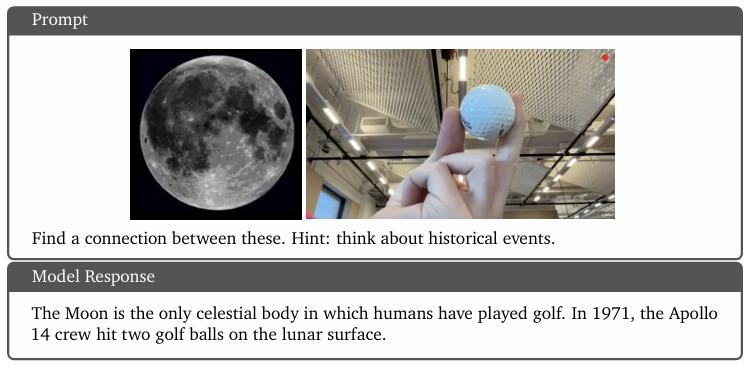
\includegraphics[width=0.9\textwidth]{gemini_multiimage_analysis.png}
    \caption{Se solicita a Gemini reconocer las imágenes y encontrar una relación entre ellas.}
    \label{fig:gemini_analysis}
\end{figure}

El sistema soporta modalidades múltiples incluyendo texto, imagen, audio y video, con capacidad de procesamiento de imágenes de hasta 30MB en formatos JPEG, PNG, GIF, WebP, PDF, SVG y HEIC. La ventana de contexto se expande masivamente a 2 millones de tokens.

Gemini 2.0 Flash integra Google Lens como módulo nativo, eliminando la arquitectura de integración externa de generaciones anteriores. El sistema demuestra precisión mejorada en estimaciones dimensionales, alcanzando márgenes de $\pm$8--15\% con objetos de referencia en productos estándar, $\pm$5--12\% en condiciones de laboratorio controlado, y $\pm$12--25\% en uso típico de usuarios reales \cite{Team20252}.

Implementaciones específicas en logística incluyen:
\begin{itemize}
    \item Análisis de inventario en tiempo real para Google Shopping
    \item Medición automatizada de productos para Google Merchant Center
    \item Optimización de embalaje en centros de distribución
    \item Análisis de fotografías de productos para Google Lens Shopping
\end{itemize}

\subsubsection{Caso 4: Vision Transformer (ViT) para reconocimiento y dimensionado de productos}

Vision Transformer (ViT), introducido por Dosovitskiy et al. en Google Research (2020) y publicado en ICLR 2021, revolucionó el campo de \textit{computer vision} al demostrar que arquitecturas transformer puras pueden superar las redes neuronales convolucionales tradicionales en tareas de reconocimiento de imágenes. El modelo alcanza 94.2\% de precisión en \textit{ImageNet classification} cuando se \textit{pre-entrena} en \textit{datasets} suficientemente grandes \cite{Dosovitskiy2020}.

La arquitectura divide imágenes en \textit{patches} de 16$\times$16 píxeles que se procesan como secuencias, similar al procesamiento de tokens en modelos de lenguaje. Esta metodología permite \textit{transfer learning} eficiente para nuevas categorías de productos.

Las implementaciones académicas posteriores han demostrado aplicabilidad directa en \textit{retail analytics}. DINOv2 (Meta AI Research, 2023) introduce \textit{self-supervised learning} que elimina la dependencia de datasets etiquetados masivos, logrando representaciones visuales robustas especialmente efectivas para reconocimiento de productos \cite{Oquab2024}.

Para estimación dimensional, las investigaciones académicas reportan precisiones de $\pm$12--18\% en objetos con referencias visuales, utilizando visual \textit{reasoning} sobre \textit{features transformer} que capturan relaciones espaciales complejas.

% ------------------------------------------------------------------
\subsection{Aplicaciones de LLMs multimodal en logística y comercio electrónico}
% ------------------------------------------------------------------

Florence (Microsoft Research, 2021) establece un framework multimodal que combina \textit{vision transformers} con capacidades de lenguaje natural, demostrando aplicabilidad directa para tareas que requieren comprensión semántica de productos y estimación de propiedades físicas.

Las evaluaciones académicas independientes confirman escalabilidad para procesamiento de millones de productos, con implementaciones que mantienen eficiencia computacional mediante técnicas de \textit{patch embedding} optimizadas.

% ------------------------------------------------------------------
\section{Características de soluciones semejantes o similares}
% ------------------------------------------------------------------

\subsection{Arquitecturas de procesamiento predominantes}

Las soluciones analizadas convergen en arquitecturas de procesamiento que combinan múltiples enfoques tecnológicos. Los sistemas comerciales líderes utilizan \textit{transformers} multimodal que integran vision encoders especializados (CLIP, ALIGN, ViT) con \textit{large language models} para interpretación semántica avanzada.

Las implementaciones actuales emplean \textit{attention mechanisms cross-modal} que permiten correlación directa entre características visuales y comprensión textual, facilitando estimación dimensional mediante razonamiento contextual \cite{Dosovitskiy2020}.

\subsection{Capacidades de interpretación dimensional}

Las capacidades de interpretación dimensional se fundamentan en:

\begin{enumerate}
    \item \textbf{Reconocimiento automático de referencias de escala}: Los modelos identifican objetos conocidos (monedas, tarjetas, manos humanas) para establecer proporciones relativas.
    \item \textbf{Análisis de perspectiva y profundidad visual}: Utiliza \textit{depth estimation} implícito derivado de características de textura y sombras.
    \item \textbf{Razonamiento contextual sofisticado}: Combina reconocimiento de objetos conocidos con análisis proporcional de elementos en la imagen \cite{Oquab2024}.
\end{enumerate}

\subsection{Precisión y confiabilidad según implementación}

La precisión varía significativamente según la implementación y condiciones operacionales:

\begin{table}[H]
\centering
\caption{Comparativa de precisión por tipo de sistema.}
\label{tab:precision_sistemas}
\begin{tabular}{@{}lcc@{}}
\toprule
\textbf{Tipo de Sistema} & \textbf{Condiciones Óptimas} & \textbf{Condiciones Reales} \\
\midrule
LLMs multimodal & $\pm$10--25\% & $\pm$15--30\% \\
Vision Transformers & $\pm$12--18\% & $\pm$15--25\% \\
Sistemas con hardware & $\pm$2--5mm & $\pm$5--10mm \\
\bottomrule
\end{tabular}
\end{table}

La degradación de precisión con iluminación deficiente, ángulos subóptimos y \textit{backgrounds} complejos representa un desafío común.

% ------------------------------------------------------------------
\section{Compendio de tecnologías, herramientas, métodos, modelos utilizados con éxito}
% ------------------------------------------------------------------

\subsection{Modelos de lenguaje multimodal predominantes}

\textbf{Modelos de gran escala comerciales:}
\begin{itemize}
    \item GPT-4 Vision (OpenAI) - 1.76 trillones de parámetros
    \item Claude Sonnet 4 (Anthropic) - Optimizado para razonamiento visual
    \item Gemini 2.0 Flash (Google) - Optimizaciones de velocidad
    \item LLaVA - Alternativas \textit{open-source}
\end{itemize}

\textbf{Arquitecturas especializadas predominantes:}
\begin{itemize}
    \item CLIP (\textit{Contrastive Language-Image Pre-training})
    \item BLIP-2 (\textit{Bootstrapped vision-language pre-training})
    \item InstructBLIP - Seguimiento de instrucciones específicas
    \item MiniGPT-4 - Eficiencia en recursos limitados
\end{itemize}

\subsection{Frameworks de visión por computadora académicos}

Vision Transformers (ViT) representan el estado del arte en análisis visual académico:

\begin{itemize}
    \item ViT-Base: 86 millones de parámetros
    \item ViT-Large: 307 millones de parámetros
    \item ViT-Huge: 632 millones de parámetros
\end{itemize}

Modelos híbridos incluyen DeiT (\textit{Data-efficient image Transformers}), Swin Transformer optimizado para imágenes de alta resolución, y EfficientViT diseñado para implementaciones móviles.

\subsection{Tecnologías de infraestructura en la nube}

\textbf{Plataformas de IA como servicio:}
\begin{itemize}
    \item OpenAI API con GPT-4 Vision endpoints
    \item Anthropic Claude API para análisis multimodal
    \item Google Vertex AI con modelos Gemini integrados
    \item Azure Cognitive Services
    \item AWS Bedrock
\end{itemize}

\textbf{Servicios de computación distribuida:}
\begin{itemize}
    \item AWS Lambda - Procesamiento \textit{serverless}
    \item Google Cloud Run - Containerización
    \item Azure Container Instances - Escalabilidad elástica
    \item Kubernetes - Orquestación de microservicios
\end{itemize}

\subsection{Herramientas de desarrollo e integración}

\textbf{Bibliotecas de integración:}
\begin{itemize}
    \item LangChain - Framework para aplicaciones LLM
    \item LlamaIndex - \textit{Retrieval-Augmented Generation}
    \item Haystack - Pipelines \textit{end-to-end}
    \item Transformers (HuggingFace) - Acceso a modelos pre-entrenados
\end{itemize}

\textbf{SDKs para desarrollo móvil:}
\begin{itemize}
    \item React Native con plugins para APIs de IA
    \item Flutter con packages para computer vision
    \item Swift/Kotlin con SDKs nativos
    \item Progressive Web Apps para acceso universal
\end{itemize}

\subsection{Metodologías de prompt engineering y optimización}

\textbf{Técnicas avanzadas de diseño de prompts:}
\begin{itemize}
    \item \textit{Few-shot learning} para medición dimensional
    \item \textit{Chain-of-thought prompting} para razonamiento paso a paso
    \item \textit{Structured output formatting} para consistencia
    \item \textit{Multi-turn conversation} para refinación iterativa
\end{itemize}

\textbf{Estrategias de optimización:}
\begin{itemize}
    \item \textit{Fine-tuning} con datos del dominio logístico
    \item \textit{Retrieval-Augmented Generation} (RAG)
    \item \textit{In-context learning} con ejemplos calibrados
    \item LoRA y Adapters para personalización eficiente
\end{itemize}

% ------------------------------------------------------------------
\section{Conjunto de características y especificaciones para la solución óptima}
% ------------------------------------------------------------------

\subsection{Arquitectura tecnológica óptima}

Basándose en el análisis de soluciones existentes, la arquitectura óptima debe combinar:

\begin{itemize}
    \item Modelos de lenguaje multimodal de última generación
    \item Infraestructura \textit{cloud} escalable
    \item Procesamiento distribuido eficiente
    \item Interfaces móviles intuitivas
\end{itemize}

\subsection{Precisión y confiabilidad requeridas}

Para aplicaciones logísticas comerciales, el sistema debe alcanzar:

\begin{itemize}
    \item Precisión de $\pm$15--20\% en condiciones reales de uso
    \item Mejora a $\pm$10--15\% con referencias de escala adecuadas
    \item Tiempos de respuesta inferiores a 5 segundos
    \item Disponibilidad superior al 99.5\%
\end{itemize}

Esta precisión es suficiente para categorización de tarifas de envío, optimización básica de carga vehicular, y estimaciones de costos logísticos sin requerir inversión en hardware especializado.

\subsection{Limitaciones y alcances reconocidos}

El sistema está diseñado para:

\begin{itemize}
    \item Estimaciones dimensionales aproximadas para categorización logística
    \item Paquetes regulares de e-commerce (5cm a 2 metros)
    \item Condiciones de iluminación mínima adecuada
    \item Mercado peruano inicialmente, con escalabilidad regional
\end{itemize}

Limitaciones reconocidas:

\begin{itemize}
    \item No apto para aplicaciones que requieran precisión milimétrica
    \item Degradación con objetos transparentes o altamente reflectivos
    \item Requiere iluminación mínima adecuada
    \item Formas extremadamente irregulares presentan mayor error
\end{itemize}
% Agrega aquí más capítulos según avances:
% % cSpell:language es,en
% ==================================================================
% CAPÍTULO 3: ESTADO DEL ARTE
% ==================================================================
\chapter{Estado del arte o de la cuestión, alternativas de solución al problema o desafío a resolver}
% \input{capitulos/04_resultados.tex}
% \input{capitulos/05_conclusiones.tex}

% ------------------------------------------------------------------
% CONCLUSIONES Y RECOMENDACIONES
% ------------------------------------------------------------------
\chapter*{Conclusiones}
\addcontentsline{toc}{chapter}{Conclusiones}
[Por completar]

\chapter*{Recomendaciones}
\addcontentsline{toc}{chapter}{Recomendaciones}
[Por completar]


% ------------------------------------------------------------------
% BIBLIOGRAFÍA
% ------------------------------------------------------------------
\cleardoublepage
\printbibliography[title={Referencias Bibliográficas}]
\addcontentsline{toc}{chapter}{Referencias Bibliográficas}

% ------------------------------------------------------------------
% ANEXOS
% ------------------------------------------------------------------
\appendix
% cSpell:language es,en
% ==================================================================
% ANEXOS DEL CAPÍTULO 3
% ==================================================================

\appendix

% ------------------------------------------------------------------
\chapter{Caracterización detallada de actores del sistema}
\label{anexo:actores}

% ------------------------------------------------------------------

\section*{Actor: Clientes (Emisores)}

\begin{table}[H]
\centering
\begin{tabular}{|p{4cm}|p{10cm}|}
\hline
\textbf{Rol en el sistema} & Usuarios que solicitan el servicio de envío de paquetes \\
\hline
\textbf{Necesidades principales} & Necesitan enviar paquetes de manera rápida y confiable sin invertir tiempo en mediciones manuales. Requieren conocer el estado de sus pedidos en tiempo real y tener transparencia en los costos del servicio. \\
\hline
\textbf{Puntos de dolor actuales} & Actualmente deben medir manualmente los paquetes o proporcionar estimaciones que pueden no corresponder con la realidad. Experimentan falta de trazabilidad durante la entrega y sufren reprogramaciones cuando los paquetes están mal estimados, generando incertidumbre sobre las condiciones del servicio. \\
\hline
\end{tabular}
\end{table}

\section*{Actor: Administradores}

\begin{table}[H]
\centering
\begin{tabular}{|p{4cm}|p{10cm}|}
\hline
\textbf{Rol en el sistema} & Gestores de la operación logística de la empresa \\
\hline
\textbf{Necesidades principales} & Buscan maximizar la eficiencia operativa atendiendo el mayor número de pedidos posible. Necesitan asignar pedidos adecuadamente a motorizados, supervisar entregas en tiempo real y poder rechazar pedidos que excedan la capacidad operativa del servicio. \\
\hline
\textbf{Puntos de dolor actuales} & Enfrentan una gestión manual de pedidos mediante WhatsApp y hojas de Excel que no escala. Carecen de visibilidad en tiempo real de la operación y tienen dificultad para validar las dimensiones reportadas por los clientes, lo que genera pérdida de eficiencia por aceptar paquetes sobredimensionados. \\
\hline
\end{tabular}
\end{table}

\section*{Actor: Motorizados (Repartidores)}

\begin{table}[H]
\centering
\begin{tabular}{|p{4cm}|p{10cm}|}
\hline
\textbf{Rol en el sistema} & Operadores de campo que recogen y entregan paquetes \\
\hline
\textbf{Necesidades principales} & Requieren recibir información clara sobre los pedidos asignados para optimizar el espacio en su mochila o cajas de reparto. Necesitan conocer rutas y ubicaciones con precisión, registrar evidencias de recojo y entrega fácilmente, y evitar viajes innecesarios por paquetes que no pueden transportar. \\
\hline
\textbf{Puntos de dolor actuales} & Experimentan sorpresas frecuentes con paquetes más grandes de lo reportado, lo que genera pérdida de tiempo y combustible en recojos no viables. Carecen de herramientas adecuadas para comunicar el estado del pedido en tiempo real y enfrentan dificultad para gestionar múltiples entregas simultáneas de manera eficiente. \\
\hline
\end{tabular}
\end{table}

\section*{Actor: Destinatarios (Receptores)}

\begin{table}[H]
\centering
\begin{tabular}{|p{4cm}|p{10cm}|}
\hline
\textbf{Rol en el sistema} & Usuarios finales que reciben los paquetes \\
\hline
\textbf{Necesidades principales} & Esperan recibir sus paquetes en el tiempo estimado y conocer cuándo llegará el motorizado. Necesitan tener confianza en el servicio y sentirse informados durante el proceso de entrega. \\
\hline
\textbf{Puntos de dolor actuales} & Sufren reprogramaciones frecuentes debido a problemas logísticos en la cadena de entrega. Experimentan falta de información sobre el estado real de su pedido y quedan insatisfechos cuando el servicio se retrasa sin explicación clara. \\
\hline
\end{tabular}
\end{table}

% ------------------------------------------------------------------
\chapter{Síntesis de hallazgos de la fase de empatía}
\label{anexo:hallazgos}
% ------------------------------------------------------------------

\section{Necesidades identificadas}

\begin{itemize}
    \item \textbf{Automatización de procesos manuales}: La medición de dimensiones de paquetes consume tiempo y genera estimaciones inexactas, mientras que la gestión de pedidos mediante WhatsApp y hojas de cálculo resulta ineficiente para escalar operaciones.
    
    \item \textbf{Visibilidad y trazabilidad en tiempo real}: Clientes requieren conocer el estado de sus envíos, administradores necesitan supervisar la operación completa, y motorizados demandan información clara sobre asignaciones y rutas.
    
    \item \textbf{Optimización de recursos limitados}: Las empresas necesitan soluciones de bajo costo con modelos de pago progresivos, y los motorizados requieren maximizar el aprovechamiento del espacio de transporte para cumplir múltiples entregas eficientemente.
\end{itemize}

\section{Restricciones del contexto}

\begin{itemize}
    \item \textbf{Restricción económica}: Presupuestos limitados para inversión tecnológica inicial y necesidad de evitar costos fijos elevados que comprometan la viabilidad del negocio.
    
    \item \textbf{Restricción técnica}: El uso predominante de dispositivos Android de gama media a baja condiciona las decisiones de diseño hacia arquitecturas que minimicen el procesamiento local. Se implementan estrategias básicas de eficiencia (compresión de imágenes, procesamiento en cloud, uso de SDKs nativos).
    
    \item \textbf{Restricción operativa}: Conectividad variable en diferentes zonas de Lima que requiere estrategias de sincronización y manejo de estados offline para garantizar continuidad del servicio.
    
    \item \textbf{Restricción normativa}: Cumplimiento obligatorio de la Ley N.º 29733 de Protección de Datos Personales en el manejo de ubicaciones, fotografías de evidencia y datos personales de usuarios.
\end{itemize}

\section{Oportunidades de mejora mediante tecnología}

\begin{itemize}
    \item \textbf{Inteligencia artificial para visión por computadora}: Automatización de estimación de dimensiones mediante fotografías con objetos de referencia, eliminando tiempo de medición manual y reduciendo errores humanos.
    
    \item \textbf{Infraestructura cloud escalable (Firebase)}: Sincronización en tiempo real entre dispositivos móviles y dashboard web sin requerir servidores físicos costosos, proporcionando trazabilidad completa de operaciones.
    
    \item \textbf{Notificaciones push (Firebase Cloud Messaging)}: Comunicación instantánea de cambios de estado a todos los actores, mejorando coordinación operativa y experiencia de usuario.
    
    \item \textbf{Geolocalización (Google Maps API)}: Optimización de rutas de entrega y seguimiento en tiempo real de motorizados, aumentando eficiencia del servicio y reduciendo tiempos de entrega.
    
    \item \textbf{Modelo de costos por uso}: Servicios cloud con pago progresional que se alinea con el crecimiento de empresas pequeñas, eliminando barreras de entrada por inversiones iniciales prohibitivas.
\end{itemize}

% ------------------------------------------------------------------
\chapter{Matriz de trazabilidad completa}
\label{anexo:trazabilidad}
% ------------------------------------------------------------------

\begin{longtable}{|p{3.5cm}|p{2.5cm}|p{2.5cm}|p{5.5cm}|}
\caption{Matriz de trazabilidad: Necesidades vs. Requerimientos.} \\
\hline
\textbf{Necesidad identificada} & \textbf{Req. funcionales} & \textbf{Req. no funcionales} & \textbf{Justificación técnica} \\
\hline
\endfirsthead

\multicolumn{4}{c}{\textit{Continuación de la tabla}} \\
\hline
\textbf{Necesidad identificada} & \textbf{Req. funcionales} & \textbf{Req. no funcionales} & \textbf{Justificación técnica} \\
\hline
\endhead

\hline
\endfoot

Automatización de medición de dimensiones & RF2.3, RF2.4 & RNF1.1, RNF6.2, RNF7.1, RNF7.2 & El módulo de IA con Cloud Functions procesa imágenes automáticamente, reduciendo tiempo de medición manual y errores humanos, con compresión optimizada para minimizar consumo de datos. \\
\hline

Trazabilidad en tiempo real de pedidos & RF2.1, RF2.5, RF3.4, RF4.1, RF5.1, RF5.2 & RNF1.2, RNF2.1 & La sincronización en tiempo real de Firestore combinada con notificaciones push proporciona visibilidad completa del estado de pedidos a todos los actores. \\
\hline

Gestión centralizada para administradores & RF4.1, RF4.2, RF4.3 & RNF1.2, RNF4.2, RNF5.1 & El dashboard web con React permite supervisión completa, filtrado eficiente y visualización geográfica de operaciones desde cualquier navegador. \\
\hline

Herramientas operativas para motorizados & RF3.1, RF3.2, RF3.3, RF3.5 & RNF4.1, RNF5.1, RNF6.1 & La aplicación Android nativa optimizada proporciona acceso eficiente a funciones del dispositivo (cámara, GPS) con bajo consumo de batería. \\
\hline

Solución de bajo costo escalable & RF1.1, RF6.1, RF6.2 & RNF2.1, RNF3.1, RNF9.1, RNF9.2 & La arquitectura serverless de Firebase elimina costos de servidores físicos y escala automáticamente con modelo de pago por uso. \\
\hline

Seguridad de información sensible & RF6.1, RF6.2 & RNF3.1, RNF3.2, RNF3.3, RNF7.1-RNF7.5 & Firebase Auth, reglas de seguridad de Firestore, cifrado SSL/TLS y cumplimiento de Ley N.º 29733 protegen datos personales y operativos. \\
\hline

Optimización de espacio de transporte & RF2.3, RF2.4, RF3.5 & RNF6.1 & Las dimensiones precisas permiten a motorizados planificar mejor la capacidad de carga y a administradores asignar pedidos compatibles. \\
\hline

Compatibilidad con dispositivos limitados & RF3.1, RF3.2, RF3.3 & RNF4.1, RNF9.1, RNF9.2 & El diseño considera dispositivos Android de gama media-baja, optimizando procesamiento, memoria y consumo de batería. \\
\hline

\end{longtable}

% ------------------------------------------------------------------
\chapter{Modelo de datos detallado}
\label{anexo:modelo-datos}
% ------------------------------------------------------------------

\section{Colección: USUARIOS}

\textbf{Ruta:} \texttt{usuarios/\{uid\}}

\begin{lstlisting}[language=json,caption={Estructura de documento Usuario}]
{
  uid: string,              // ID unico de Firebase Auth
  email: string,            // Correo electronico
  phone: string,            // Telefono de contacto
  nombre: string,           // Nombre del usuario
  apellido: string,         // Apellido del usuario
  rol: string,              // 'administrador' | 'cliente' | 'motorizado'
  
  // Datos especificos para clientes empresariales (opcional)
  datosEmpresariales: {
    nombreEmpresa: string,
    ruc: string,
    razonSocial: string
  } | null,
  
  // Datos especificos para motorizados (opcional)
  datosMotorizado: {
    estadoServicio: string, // 'disponible' | 'ocupado' | 'desconectado'
    vehiculo: {
      placa: string,
      tipo: string,         // 'motocicleta' | 'bicicleta' | 'auto'
      modelo: string,
      anio: number
    },
    estadisticas: {
      pedidosCompletados: number,
      calificacionPromedio: number,
      tiempoPromedioEntrega: number  // en minutos
    }
  } | null,
  
  // Ultima ubicacion conocida (para motorizados)
  ultimaUbicacionConocida: {
    latitud: number,
    longitud: number,
    timestamp: timestamp,
    distrito: string
  } | null,
  
  // Metadatos
  creadoEn: timestamp,
  actualizadoEn: timestamp,
  activo: boolean,
  ultimaConexion: timestamp
}
\end{lstlisting}

\section{Colección: PEDIDOS}

\textbf{Ruta:} \texttt{pedidos/\{pedidoId\}}

\begin{lstlisting}[language=json,caption={Estructura de documento Pedido (parte 1)}]
{
  id: string,  // ID unico del pedido
  
  // Estructura de asignacion (recojo y entrega pueden ser diferentes)
  asignacion: {
    recojo: {
      estado: string,       // 'pendiente' | 'asignado' | 'completado'
      rutaId: string | null,
      rutaNombre: string | null,
      motorizadoUid: string | null,
      motorizadoNombre: string | null,
      asignadaEn: timestamp | null,
      razonPendiente: string | null
    },
    entrega: {
      // Estructura similar a recojo
    }
  },
  
  // Control de visibilidad por rol
  visibilidad: {
    motorizadoRecojo: boolean,
    motorizadoEntrega: boolean,
    administrador: boolean
  },
  
  // Ciclo operativo del pedido
  cicloOperativo: {
    diaCreacion: string,    // YYYY-MM-DD
    diaAsignado: string,
    cerradoPorAdmin: boolean,
    fechaCierreAdmin: timestamp | null,
    horaLimiteRecojo: timestamp,
    permiteEntregaAntes13h: boolean
  },
  
  // Indices para consultas eficientes
  indices: {
    requiereAsignacionManual: boolean,
    motorizadoRecojoUid: string | null,
    motorizadoEntregaUid: string | null,
    rutaRecojoId: string | null,
    rutaEntregaId: string | null,
    distritoRecojo: string,
    distritoEntrega: string
  }
}
\end{lstlisting}

\begin{lstlisting}[language=json,caption={Estructura de documento Pedido (parte 2)}]
{
  // Informacion del proveedor (quien envia)
  proveedor: {
    uid: string,
    nombre: string,
    correo: string,
    telefono: string,
    direccion: {
      link: string,         // URL de Google Maps
      distrito: string,
      coordenadas: {
        latitud: number,
        longitud: number
      }
    }
  },
  
  // Informacion del destinatario (quien recibe)
  destinatario: {
    nombre: string,
    telefono: string,
    direccion: {
      link: string,
      distrito: string,
      coordenadas: {
        latitud: number,
        longitud: number
      }
    }
  },
  
  // Informacion del paquete
  paquete: {
    detalle: string,        // Descripcion del contenido
    observaciones: string,
    dimensiones: {
      alto: number,         // en centimetros
      ancho: number,
      largo: number,
      volumen: number,      // calculado automaticamente
      peso: number | null,  // opcional
      estimadoPorIA: boolean,
      editadoManualmente: boolean,
      excedeMaximo: boolean,
      confianzaIA: number | null  // 0-1, nivel de confianza del modelo
    },
    fotos: {
      recojo: {
        url: string,
        thumbnail: string,
        timestamp: timestamp,
        procesadaPorIA: boolean
      },
      entrega: {
        url: string,
        thumbnail: string,
        timestamp: timestamp
      },
      comprobantePago: {
        url: string,
        thumbnail: string,
        timestamp: timestamp
      }
    }
  }
}
\end{lstlisting}

\begin{lstlisting}[language=json,caption={Estructura de documento Pedido (parte 3)}]
{
  // Informacion de pago
  pago: {
    seCobra: boolean,
    metodoPago: string,     // 'efectivo' | 'transferencia' | 'yape' | 'plin'
    monto: number,
    comision: number,
    montoTotal: number,
    estadoPago: string,     // 'pendiente' | 'pagado' | 'por_cobrar'
    billeteraUsada: {
      id: string,
      propietarioTipo: string,  // 'proveedor' | 'empresa'
      metodo: string,
      titular: string
    }
  },
  
  // Informacion del motorizado asignado (desnormalizado)
  motorizado: {
    uid: string,
    nombre: string,
    asignadoEn: timestamp,
    aceptadoEn: timestamp | null
  } | null,
  
  // Fechas del ciclo de vida del pedido
  fechas: {
    creacion: timestamp,
    entregaProgramada: timestamp,
    recojo: timestamp | null,
    entrega: timestamp | null,
    anulacion: timestamp | null
  },
  
  // Control de version para actualizaciones concurrentes
  actualizadoEn: timestamp,
  version: number
}
\end{lstlisting}

\section{Colección: BILLETERAS}

\textbf{Ruta:} \texttt{billeteras/\{billeteraId\}}

\begin{lstlisting}[language=json,caption={Estructura de documento Billetera}]
{
  id: string,
  propietario: {
    tipo: string,           // 'proveedor' | 'empresa'
    uid: string | null,     // Si es proveedor, referencia a usuario
    nombreEmpresa: string
  },
  alias: string,            // Nombre descriptivo
  metodo: string,           // 'yape' | 'plin' | 'transferencia_bancaria'
  cuenta: {
    titular: string,
    telefono: string,       // Para Yape/Plin
    numeroDocumento: string | null,  // DNI/RUC
    tipoDocumento: string | null     // 'DNI' | 'RUC'
  },
  qr: {
    urlImagen: string,      // URL de Firebase Storage
    urlImagenThumbnail: string | null,
    hash: string | null     // Para validacion
  },
  config: {
    activo: boolean,
    porDefecto: boolean,
    soloEfectivo: boolean,
    limiteMaximo: number | null,
    comisionPorcentaje: number,
    prioridad: number       // Para ordenar opciones
  },
  verificado: boolean,
  verificadoPor: {
    uid: string,
    nombre: string,
    fecha: timestamp
  },
  creadoEn: timestamp,
  actualizadoEn: timestamp,
  ultimoUso: timestamp | null,
  totalTransacciones: number
}
\end{lstlisting}

\subsection{Índices compuestos necesarios}

\begin{itemize}
    \item \texttt{proveedor.uid + fechas.creacion} (pedidos por cliente)
    \item \texttt{motorizado.uid + fechas.creacion} (pedidos por motorizado)
    \item \texttt{asignacion.recojo.estado + cicloOperativo.diaCreacion} (pedidos pendientes del día)
    \item \texttt{indices.distritoEntrega + fechas.entregaProgramada} (optimización de rutas)
\end{itemize}

% ------------------------------------------------------------------
\chapter{Configuración de seguridad y autenticación}
\label{anexo:seguridad}
% ------------------------------------------------------------------

\section{Estructura de custom claims}

\begin{lstlisting}[language=json,caption={Custom claims en Firebase Authentication}]
{
  rol: 'administrador' | 'cliente' | 'motorizado',
  permisos: ['crear_pedido', 'asignar_motorizado', 'ver_dashboard'],
  empresaId: string | null  // Para clientes empresariales
}
\end{lstlisting}

\section{Reglas de seguridad de Firestore}

\begin{lstlisting}[caption={Firestore Security Rules}]
rules_version = '2';
service cloud.firestore {
  match /databases/{database}/documents {
    // Funcion helper para verificar autenticacion
    function isAuthenticated() {
      return request.auth != null;
    }
    
    // Funcion helper para verificar rol
    function hasRole(role) {
      return isAuthenticated() && 
             request.auth.token.rol == role;
    }
    
    // Usuarios: pueden leer/actualizar su propio perfil
    match /usuarios/{userId} {
      allow read: if isAuthenticated() && 
                     (request.auth.uid == userId || 
                      hasRole('administrador'));
      allow write: if isAuthenticated() && 
                      request.auth.uid == userId;
      allow create: if hasRole('administrador');
    }
    
    // Pedidos: acceso segun rol
    match /pedidos/{pedidoId} {
      allow read: if isAuthenticated() && (
        hasRole('administrador') ||
        (hasRole('cliente') && 
         resource.data.proveedor.uid == request.auth.uid) ||
        (hasRole('motorizado') && 
         resource.data.motorizado.uid == request.auth.uid)
      );
      
      allow create: if isAuthenticated() && 
                       (hasRole('administrador') || 
                        hasRole('cliente'));
      
      allow update: if isAuthenticated() && (
        hasRole('administrador') ||
        (hasRole('motorizado') && 
         resource.data.motorizado.uid == request.auth.uid)
      );
      
      allow delete: if hasRole('administrador');
    }
    
    // Billeteras: solo administradores y propietarios
    match /billeteras/{billeteraId} {
      allow read: if isAuthenticated();
      allow write: if hasRole('administrador') || 
                      resource.data.propietario.uid == request.auth.uid;
    }
  }
}
\end{lstlisting}

\section{Reglas de seguridad de Storage}

\begin{lstlisting}[caption={Firebase Storage Security Rules}]
rules_version = '2';
service firebase.storage {
  match /b/{bucket}/o {
    // Helper functions
    function isAuthenticated() {
      return request.auth != null;
    }
    
    function hasRole(role) {
      return isAuthenticated() && 
             request.auth.token.rol == role;
    }
    
    // Imagenes de pedidos
    match /pedidos/{pedidoId}/{tipo}/{filename} {
      allow read: if isAuthenticated();
      allow write: if isAuthenticated() && (
        hasRole('administrador') ||
        hasRole('cliente') ||
        hasRole('motorizado')
      );
    }
    
    // Fotos de perfil
    match /usuarios/{userId}/{filename} {
      allow read: if isAuthenticated();
      allow write: if isAuthenticated() && 
                      request.auth.uid == userId;
    }
    
    // QR de billeteras
    match /billeteras/{billeteraId}/{filename} {
      allow read: if isAuthenticated();
      allow write: if hasRole('administrador');
    }
  }
}
\end{lstlisting}

% ------------------------------------------------------------------
\chapter{Justificación de puntuaciones en matriz multicriterio}
\label{anexo:justificacion-puntuaciones}
% ------------------------------------------------------------------

\section{Escalabilidad}

\begin{itemize}
    \item \textbf{Firebase (5)}: Escalamiento automático sin configuración, maneja desde 0 hasta millones de usuarios transparentemente.
    
    \item \textbf{AWS (4)}: Excelente escalabilidad pero requiere configuración de Auto Scaling y gestión de capacidad.
    
    \item \textbf{Backend propio (2)}: Requiere planificación manual y redimensionamiento de servidores.
\end{itemize}

\section{Costo}

\begin{itemize}
    \item \textbf{Firebase (5)}: Capa gratuita generosa, ideal para desarrollo de tesis y etapas iniciales de empresas pequeñas.
    
    \item \textbf{AWS (3)}: Capa gratuita limitada a 12 meses, costos variables pero competitivos.
    
    \item \textbf{Backend propio (3)}: Costos fijos predecibles pero presentes desde el inicio.
\end{itemize}

\section{Facilidad de integración}

\begin{itemize}
    \item \textbf{Firebase (5)}: Componentes nativamente integrados, SDKs optimizados, despliegue con un comando.
    
    \item \textbf{AWS (3)}: Requiere integrar múltiples servicios manualmente, configuración compleja.
    
    \item \textbf{Backend propio (2)}: Integración completamente manual de cada componente.
\end{itemize}

\section{Mantenimiento}

\begin{itemize}
    \item \textbf{Firebase (5)}: Gestión de infraestructura completamente delegada a Google.
    
    \item \textbf{AWS (3)}: Gestión parcial, requiere actualización de componentes y monitoreo.
    
    \item \textbf{Backend propio (2)}: Responsabilidad total del mantenimiento, actualizaciones de seguridad, backups.
\end{itemize}

\section{Rendimiento}

\begin{itemize}
    \item \textbf{Firebase (4)}: Excelente para operaciones en tiempo real, latencia baja en sincronización.
    
    \item \textbf{AWS (4)}: Rendimiento configurable según recursos asignados, muy bueno con optimización.
    
    \item \textbf{Backend propio (3)}: Depende del proveedor de hosting y configuración manual.
\end{itemize}

\section{Ecosistema y soporte}

\begin{itemize}
    \item \textbf{Firebase (5)}: Documentación excelente, amplia comunidad, tutoriales especializados.
    
    \item \textbf{AWS (5)}: Documentación exhaustiva, soporte empresarial, ecosistema maduro.
    
    \item \textbf{Backend propio (3)}: Depende de múltiples fuentes, documentación fragmentada.
\end{itemize}

\end{document}